\subsection*{Senyal del far}
\addcontentsline{toc}{subsection}{Senyal del far}


La comunicació mitjançant llum visible té una llarga història, encara que la tecnologia VLC basada en LED es va inventar al segle XXI. 

\begin{figure}[h!]
    \centering
    \includegraphics[width=80mm]{comunicacióLlum.png}
    \caption{Comunicació a través del llum}
\end{figure}


\subsection*{1841: Descubriment de Reflexió total}
\addcontentsline{toc}{subsection}{1841: Descubriment de Reflexió total}

La reflexió total és el fenomen físic que es produeix quan un raig de llum incideix amb un angle superior a l'angle crític en una superfície transparent d'índex de refracció alt. Per angles d'incidència majors o iguals a l'angle crític, tota l'energia és reflectida cap al medi incident.
S'utilitza en la fibra òptica, fent que l'índex de refracció de l'interior sigui més gran que l'aire. D'aquesta manera un raig que emetem des del principi no surt del fil fins que no es talla. Es pot utilitzar per les telecomunicacions o per la cirurgia.

\begin{figure}[h!]
    \centering
    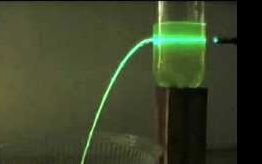
\includegraphics[width=80mm]{refluxiototal.png}
    \caption{Teoría reflexió total}
\end{figure}


Capa física de fibra: 
\begin{itemize}
    \item 1887: El científic britànic Charles va fabricar fibra de vidre per primera vegada
    \item 1938: Dues empreses nord-america i japonés van poder fabricar dibra de vidres més llargues
    \item 1956: un estudiant de la Universitat de Michigan va utilitzar un tub de vidre de baix índex de refracció i el va fondre en una vareta de vidre d'alt índex de refracció, creant la primera fibra òptica revestida de vidre. 

\end{itemize}

Defeneix utilitat de la fibra:
\begin{itemize}
    \item 1966: Físic Charles Kuen Kao es van posar les bases de les comunicacions de fibra òptica.
    \item 1971: Es llança la primera fibra òptica d'un quilòmetre de llargada
    \item 1981: Es comença el sistema de comunicació de fibra òptica 
\end{itemize}



\subsection*{Primer LED Li-Fi}
\addcontentsline{toc}{subsection}{Primer LED Li-Fi}

La tecnologia Li-Fi va ser proposada per primera vegada pel professor Harald Haas de la Universitat d'Edimburg durant una conferència TED Talk al juliol de 2011. En aquesta presentació, el professor Haas va descriure la possibilitat d'utilitzar la llum LED per a transmetre dades de manera inalàmbrica, una idea que va conduir al desenvolupament de la tecnologia Li-Fi.

Els sistemes de posicionament interior basats en VLC s'han convertit en un tema atractiu. La investigació d'ABI preveu que podria ser una solució clau per desbloquejar el "mercat d'ubicació interior" de 5.000 milions de dòlars. Les publicacions han estat provinents del laboratori Nakagawa, ByteLight va presentar una patent sobre un sistema de posicionament de llum que utilitzava el reconeixement de polsos digitals LED el març de 2012. COWA a Penn State i altres investigadors d'arreu del món.


\subsection*{Altres treball recents}
\addcontentsline{toc}{subsection}{Altres treballs recents}


\begin{itemize}
    \item Una altra aplicació és en el món de les joguines, gràcies a la implementació rendible i de baixa complexitat, que només requereix un microcontrolador i un LED com a frontal òptic.
    \item Els VLC es poden utilitzar per proporcionar seguretat. Són especialment útils en xarxes de sensors corporals i xarxes d'àrea personal.
    \item L'octubre de 2014, Axrtek va llançar un sistema comercial bidireccional RGB LED VLC anomenat MOMO que transmet cap avall i cap amunt a velocitats de 300 Mbit/s i amb un abast de 25 peus.
    \item El maig de 2015, Philips va col·laborar amb l'empresa de supermercats Carrefour per oferir serveis basats en la localització de VLC als telèfons intel·ligents dels compradors en un hipermercat de Lille, França. El juny de 2015, dues empreses xineses, Kuang-Chi i Ping An Bank, es van associar per introduir una targeta de pagament que comunica informació mitjançant una llum visible única. El març de 2017, Philips va establir els primers serveis basats en la ubicació VLC per als telèfons intel·ligents dels compradors a Alemanya. La instal·lació es va presentar a l'EuroShop de Düsseldorf (5-9 de març). Com a primer supermercat a Alemanya, un supermercat Edeka a Düsseldorf-Bilk està utilitzant el sistema, que ofereix una precisió de posicionament de 30 centímetres que es pot aconseguir, que compleix les demandes especials de la venda al detall d'aliments. Els sistemes de posicionament interior basats en VLCes poden utilitzar en llocs com hospitals, residències de gent gran, magatzems i oficines grans i obertes per localitzar persones i controlar vehicles robòtics interiors.
\end{itemize}